\section{Discussion}
Dimensionality reduction is an essential step for downstream analysis such as clustering and trajectory inference. Because of the high dimensionality and high sparsity of the single cell sequencing data, conventional clustering methods usually have poor performance on high dimensional data. Therefore, scRNA-seq data needs to be presented in a lower dimensional space by reducing the dimensionality to enable the clustering process. The traditional pipelines usually perform dimensionality reduction and clustering as separate parts \cite{wu2020tools}. However, some researches recently shows that performing dimensionality reduction and clustering jointly can achieve better results of both clustering and dimensionality reduction \cite{yang2017towards}. For example, some researchers use Gussian mixture model to cluster images when performing variational autoencoder to reduce the dimensionality of those images \cite{prasad2020variational}. Such methods that uses deep learning to aid clustering tasks are called deep clustering.

For scRNA-seq data, we can also perform deep clustering to improve the performance of clustering and dimensionality reduction. Because there are usually several cell types in a scRNA-seq dataset, in the latent space, those cell types should fall into clusters naturally. For scRNA-seq analysis, we hope to distinguish those clusters by dimensionality reduction and clustering. In this case, we can perform deep clustering methods to cluster cells and reduce the dimensionality of data at the same time. By doing so, we can not only get nice clustering results but also get a great visualization result that have greatly separated clusters that enable us to identify cell sub-populations clearly \cite{tian2019clustering}. 

We performed deep clustering by applying the clustering algorithms to the two dimensional latent variables of variational autoencoder. The basic structure are as Figure \ref{dcstru}. 

\begin{figure}
    \centering
    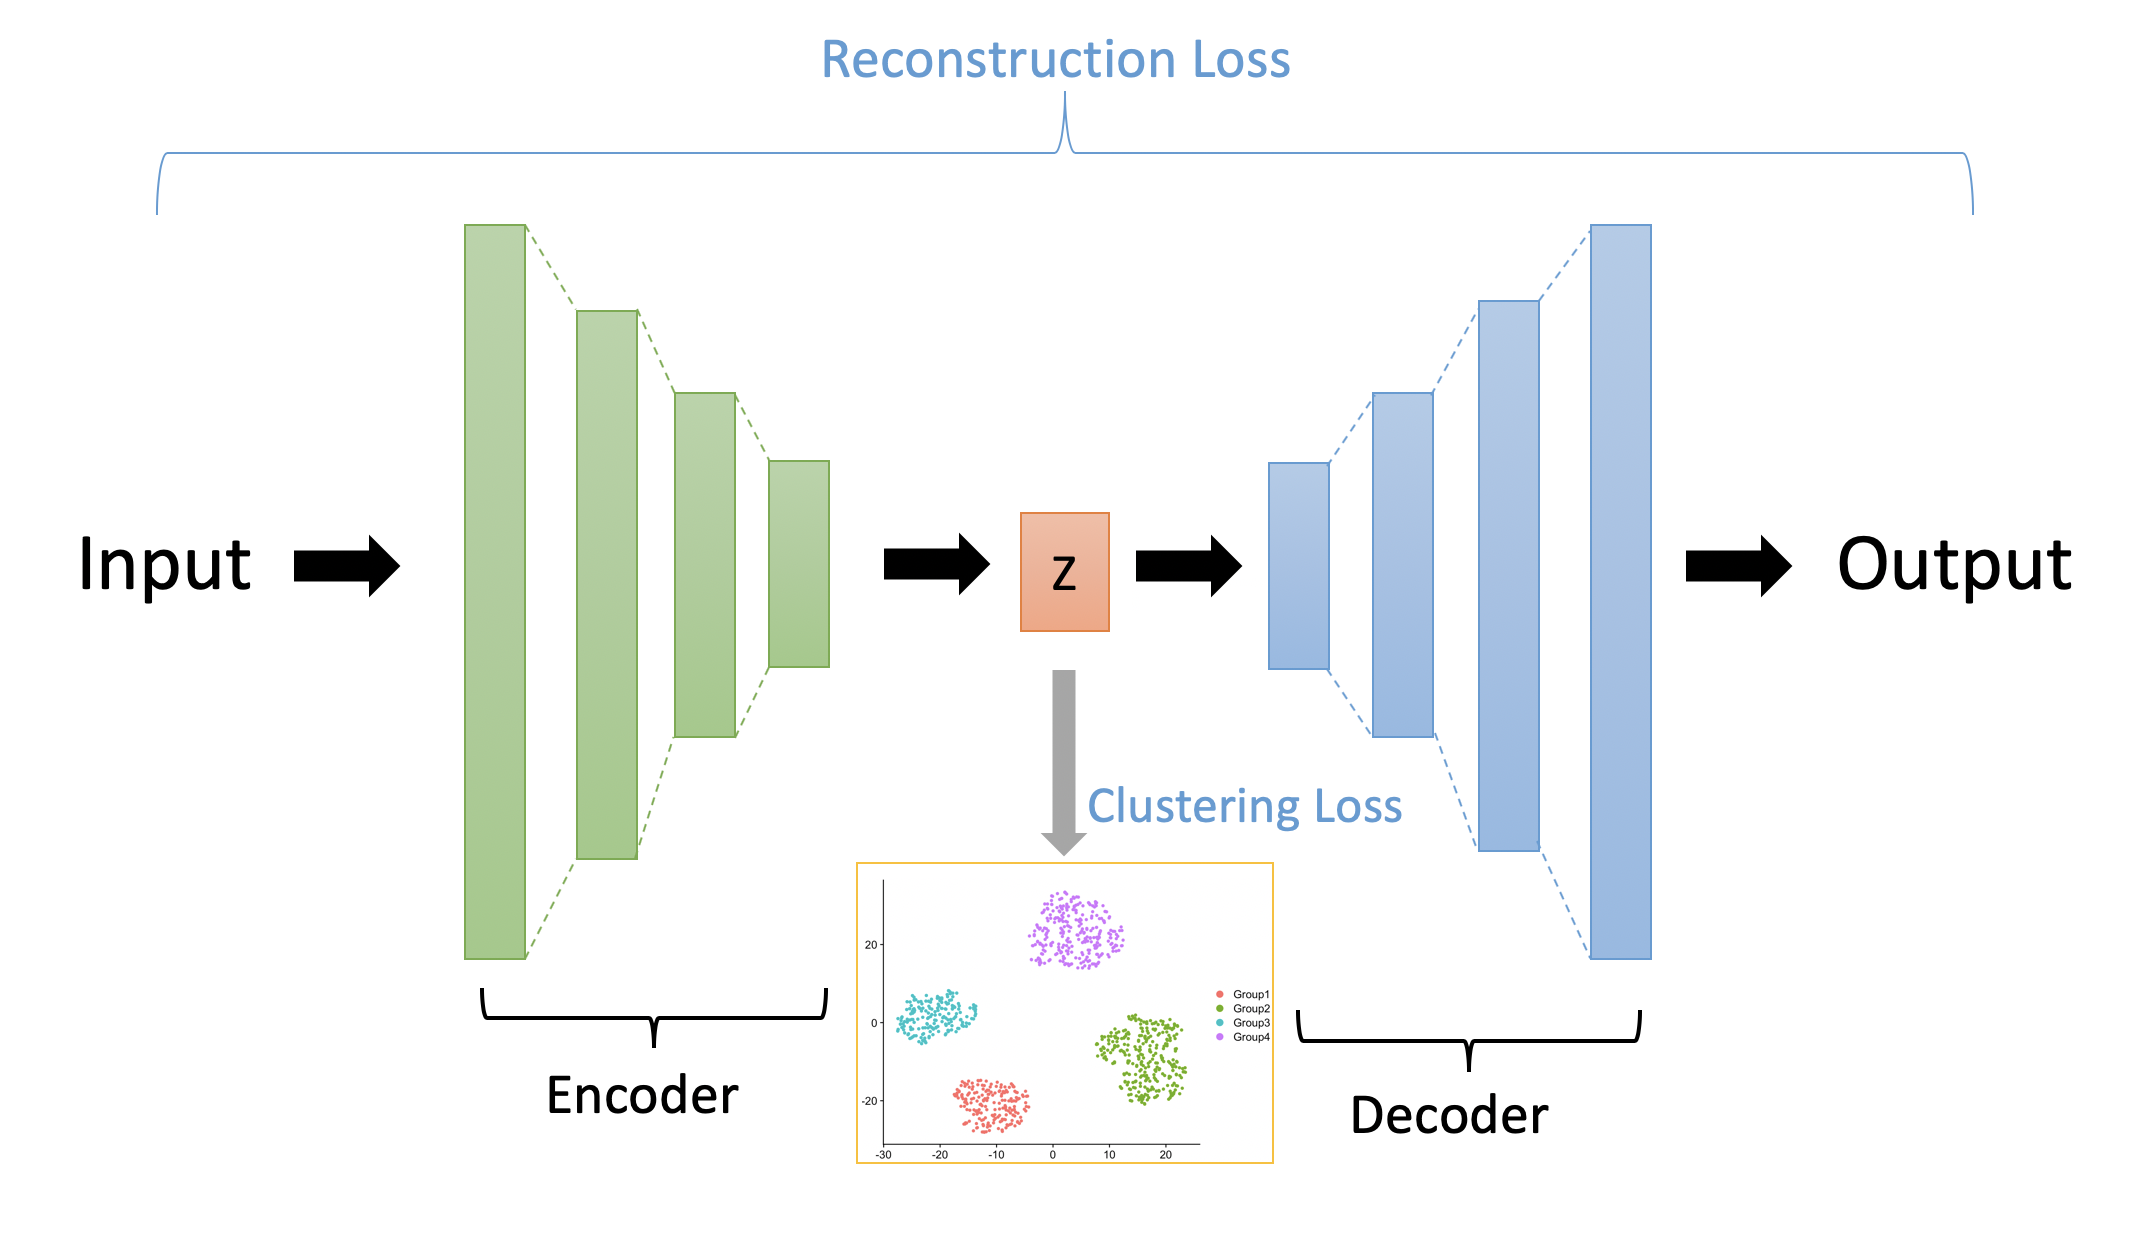
\includegraphics[width=1\textwidth]{figures/myfigures/dc.png}
    \caption{The structure of the deep clustering model}
    \label{dcstru}
\end{figure}

For the clustering process, we tried four methods: the spectral clustering \cite{von2007tutorial}, DBSCAN \cite{ester1996density}, K-means \cite{kanungo2002efficient} and louvain methods \cite{traag2019louvain}.